\chapter{Grundlagen}
\label{grundlagen}

Das folgende Kapitel erläutert die Grundlagen und Notationen, die zum weiteren Verständnis der Arbeit benötigt werden.
Zunächst werden in Unterkapitel~\ref{mathematische_notationen} die grundlegenden Notationen zu Mengen, Vektoren, Matrizen und Tensoren definiert, die im weiteren Verlauf verwendet werden.
Daraufhin folgt in Unterkapitel~\ref{graphentheorie} eine kurze Einführung in das Gebiet der Graphentheorie.
Abschließend führt das Unterkapitel~\ref{convolutional_neural_networks} in das Gebiet der neuronalen Netze und insbesondere der Convolutional Neural Networks ein, auf denen diese Arbeit aufbaut.
Für einen umfassenderen Blick in das Gebiet des \emph{Deep Learnings}, den diese Arbeit nicht leisten kann, sei auf \citeauthor{Nielsen}~\cite{Nielsen} verwiesen.

\section{Mathematische Notationen}
\label{mathematische_notationen}

\paragraph{Vektoren}
skalarprodukt

\paragraph{Matrizen}
Diagonalmatrix

\paragraph{Dünnbesetzte Matrizen}

Eine \emph{dünnbesetzte} oder \emph{schwachbesetzte Matrix} ist eine Matrix, bei der so viele Einträge aus Nullen bestehen, dass sich statt der üblichen Speicherung einer Matrix als zweidimensionales Feld speichereffizientiere Datenstrukturen ergeben.
In der Regel gilt eine Matrix $\ma{M}\in \gls{R}^{N \times N}$ als dünnbesetzt, wenn diese nicht aus mehr als $N$ oder $N \log N$ Einträgen ungleich Null besteht.
Neben dem Speichergewinn lassen sich viele Operationen auf Matrizen ebenso berechnungseffizienter implementieren~\cite{Saad}.
So muss \zB{} zur Bestimmung des größten Elements einer Matrix nicht die komplette Matrix, sondern lediglich deren explizit eingetragene Werte betrachtet werden.
Es gibt jedoch auch Operationen, die nicht auf dünnbesetzten Matritzen definiert sind, sodass diese vorher in eine \emph{dichte} Matrix überführt werden müssen (\vgl{}~\cite{Saad}).
Im Laufe dieser Arbeit haben wir es oft mit dünnbesetzten Matrizen zu tun.
So wird \zB{} eine Diagonalmatrix \emph{immer} als eine dünnbesetzte Matrix implementiert.

\paragraph{Tensoren}
Tensor, was bedeutet z.B. $\gls{W}_i$

\paragraph{Bilder}

Ein \emph{Bild} kann folglich durch einen dreidimensionalen Tensor $\gls{B} \in \gls{R}^{H \times W \times C}$ repräsentiert werden, wobei $H, W \in \gls{N}$ die Höhe \bzw{} Breite des Bildes angeben und $C \in \left\{1, 3\right\}$ die Anzahl der Farbkanäle des Bildes beschreibt, \dhe{} ein Graubild mit nur einem Kanal oder ein Farbbild mit drei Kanälen (\zB{} über das RGB- oder Lab-Farbmodell).
Ein \emph{Pixel} eines Bildes \gls{B} an der Position $\left(x, y\right), 1 \leq x \leq W, 1 \leq y \leq H$ kann folglich über $\gls{B}_{yx} \in \gls{R}^C$ angesprochen werden.

\paragraph{Mengen}

Eine ungeordnete Menge $\mathcal{A} = {\left\{a\right\}}_{n=1}^N \coloneqq \left\{a_1, \ldots, a_N\right\}$ mit $N$ Elementen, $a_n \in \mathcal{A}$.
Geordnete Menge $\left(\right)$
Eine geordnete Menge kann ebenso als Vektor, Matrix \bzw{} Tensor je nach Dimensionalität der Daten verstanden werden.

\section{Spektrale Graphentheorie}
\label{spektrale_graphentheorie}

Es gibt 2 große Quellen hier:
\begin{itemize}
  \item Spectral Graph Theory by Chung
  \item Discrete Laplace-Beltrami Operator
\end{itemize}
+ 5 zum Lernen:
\begin{itemize}
  \item Semi Supervised Classification
  \item Fast Localized Spectral Filterung
  \item Wavelets on Graphs via Spectral Graph Theory
  \item The Emerging Field of Signal Processing on Graphs
  \item How powerful are Graph Convolutions? (Review)
\end{itemize}

\subsection{Eigenwerte und Eigenvektoren reell symmetrischer Matrizen}
\label{eigenwerte_symmetrischer_matrizen}

\todo{intro}

$\ma{M} \in \gls{R}^{N \times N}$.
$\gls{eiv} \in \gls{R}^{N}$, $\gls{eiv} \neq \mathbf{0}$.
$\gls{lambda} \in \gls{R}$.
\emph{Eigenwertproblem} $\ma{M}\gls{eiv} = \gls{lambda}\gls{eiv}$.
Zu einem \emph{Eigenwert} $\gls{lambda}$ gibt es unendlich viele (skalierte) \emph{Eigenvektoren} \gls{eiv}.
Wir definieren den Eigenvektor \gls{eiv} eines Eigenwertes \gls{lambda} daher eindeutig über die Bedingung $\left\|\gls{eiv}\right\|_2 = 1$.
Sei \ma{M} weiterhin symmetrisch, \dhe{} $\ma{M} = \ma{M}^{\top}$.
Dann gilt für zwei unterschiedliche Eigenvektoren $\gls{eiv}_1$ und $\gls{eiv}_2$, dass $\gls{eiv}_1 \gls{ortho} \gls{eiv}_2$.
Weiterhin hat \ma{M} genau $N$ reelle Eigenwerte mit ${\left\{\gls{lambda}_i\right\}}_{i=1}^N$.

Wir definieren zu \ma{M} die orthogonale \emph{Eigenvektormatrix} $\gls{Eiv} \coloneqq \left[\gls{eiv}_1, \ldots, \gls{eiv}_n\right] \in \gls{R}^{N \times N}$, wobei $\gls{Eiv}\gls{Eiv}^{\top}=\gls{I}$, und dessen korrespondierende Eigenwertdiagonalmatrix $\gls{Lambda} \coloneqq \gls{diag}\left({\left[\gls{lambda}_1, \ldots, \gls{lambda}_N\right]}^{\top}\right)$, \dhe{} $\gls{Lambda}_{ii} = \gls{lambda}_i$.
Dann gilt $\ma{M}\gls{Eiv} = \gls{Eiv}\gls{Lambda}$ und insbesondere ist \ma{M} diagonalisierbar über
\begin{equation*}
  \ma{M} = \ma{M}\gls{Eiv}\gls{Eiv}^{\top} = \gls{Eiv}\gls{Lambda}\gls{Eiv}^{\top}.
\end{equation*}

Weiterhin gilt für die $k$te Potenz von $\ma{M}$, $k \in \gls{N}$,
\begin{equation}
  \ma{M}^k = {\left(\gls{Eiv}\gls{Lambda}\gls{Eiv}^{\top}\right)}^k = \gls{Eiv}\gls{Lambda}^k\gls{Eiv}^{\top}.
  \label{eq:matrix_potenz}
\end{equation}

Dieser Zusammenhang lässt sich verdeutlichen, wenn man die Potenz ausschreibt:
\begin{equation*}
  {\left(\gls{Eiv}\gls{Lambda}\gls{Eiv}^{\top}\right)}^k = \gls{Eiv}\gls{Lambda}\gls{Eiv}^{\top}\gls{Eiv}\gls{Lambda}\gls{Eiv}^{\top}\prod^{k-2}_{i=1} \gls{Eiv}\gls{Lambda}\gls{Eiv}^{\top} = \gls{Eiv}\gls{Lambda}^2\gls{Eiv}^{\top} \prod^{k-2}_{i=1} \gls{Eiv}\gls{Lambda}\gls{Eiv}^{\top} = \gls{Eiv}\gls{Lambda}^k \gls{Eiv}^{\top}.
\end{equation*}

Falls \ma{M} weiterhin \emph{schwach diagonaldominant} ist, \dhe{}
\begin{equation}
  \sum_{\substack{j=1\\j \neq i}}^N \left|\ma{M}_{ij}\right| \leq \left|\ma{M}\right|_{ii},
  \label{eq:schwach_diagonaldominant}
\end{equation}
und weiterhin $\ma{M}_{ii} \geq 0$ für alle $i \in \left\{1, \ldots, N\right\}$, dann ist \ma{M} \emph{positiv semidefinit}, \dhe{} $\ve{x}^{\top}\ma{M}\ve{x} \geq 0$ für alle $\ve{x} \in \gls{R}^{N}$.
Eigenwerte symmetrischer positiv semidefiniter Matrizen $\lambda_i \in \gls{R+}$ sind positiv reell und es lässt sich folglich auf diesen eine Ordnung definieren mit $0 \leq \gls{lambda}_1 \leq \cdots \leq \gls{lambda}_N \coloneqq \gls{lambdamax}$.

\todo{quelle}

\subsection{Laplace-Matrix}
\label{laplace_matrix}

Our eigenvalues relate well to other graph invariants for general graphs in a way that other definitions (such as the eigenvalues of adjacency matrices) often fail to do.
The advantages of this definition are perhaps due to the fact that it is consistent with the eigenvalues in spectral geometry and in stochastic processes.
Many results which were only known for regular graphs can be generalized to all graphs~\cite{Chung}.

\todo{intro}

Für einen schleifenlosen, ungerichteteten, gewichtet oder ungewichteten Graphen \gls{G} und dessen Adjazenzmatrix \gls{A} mit Gradmatrix \gls{D} ist die \emph{kombinatorische Laplace-Matrix} \gls{L} definiert als $\gls{L} \coloneqq \gls{D} - \gls{A}$~\cite{Chung}.
Die \emph{normalisierte Laplace-Matrix} \gls{Lnorm} ist definiert als $\gls{Lnorm} \coloneqq \gls{D}^{-\frac{1}{2}} \gls{L} \gls{D}^{-\frac{1}{2}}$ mit der Konvention, dass $\gls{D}^{-\frac{1}{2}}_{ii} = 0$ für isolierte Knoten $\gls{v}_i \in \gls{V}$ in \gls{G}, \dhe{} $\gls{D}_{ii} = 0$~\cite{Chung}.
Daraus ergibt sich die elementweise Definition
\begin{equation*}
  \gls{Lnorm}_{ij} \coloneqq \begin{cases}
  1, & \text{wenn }i = j,\\
    -\frac{\gls{w}\left(\gls{v}_i, \gls{v}_j\right)}{\sqrt{\gls{d}\left(\gls{v}_i\right)\gls{d}\left(\gls{v}_j\right)}}, & \text{wenn }\gls{v}_i \gls{adj} \gls{v}_j,\\
  0, & \text{sonst.}
\end{cases}
\end{equation*}
Für verbundene Graphen kann \gls{Lnorm} vereinfacht werden zu $\gls{Lnorm} \coloneqq \gls{I} - \gls{D}^{-\frac{1}{2}} \gls{A} \gls{D}^{-\frac{1}{2}}$~\cite{Chung}.
Jeder Eintrag auf der Diagonalen der normalisierten Laplace-Matrix ist folglich Eins.
\gls{Lnorm} ist damit normalisiert auf den (gewichteten) Grad zweier adjazenter Knoten $\gls{v}_i$ und $\gls{v}_j$.
Es ist anzumerken, dass \gls{L} und insbesondere \gls{Lnorm} symmetrisch sind, wohingegen eine Normalisierung der Form $\gls{D}^{-1}\gls{L}$ dies in der Regel nicht wäre~\cite{Reuter}.

\gls{L} und \gls{Lnorm} sind keine ähnlichen Matrizen.
Insbesondere sind ihre Eigenvektoren unterschiedlich.
Die Nutzung von \gls{L} oder \gls{Lnorm} ist damit abhängig von dem Problem, welches man betrachtet~\cite{Hammond}.
Wir schreiben \gls{Lboth} wenn die Wahl der Laplace-Matrix, ob \gls{L} oder \gls{Lnorm}, für die weitere Berechnung zwar fest, aber irrelevant ist.

\paragraph{Interpretation}
\label{laplace_interpretation}

\todo{kurz laplace beltrami}

Sei $\ve{f} \in \gls{R}^N$ eine Funktion \bzw{} ein Signal auf den Knoten eines Graphen \gls{G}.
Dann kann für die kombinatorische Laplace-Matrix \gls{L} verifiziert werden, dass \gls{L} die Gleichung
\begin{equation*}
  {\left(\gls{L}\ve{f}\right)}_i = \sum_{i \gls{adj} j} \gls{w}\left(\gls{v}_i, \gls{v}_j\right) \left(\ve{f}_i - \ve{f}_j\right)
\end{equation*}
erfüllt~\cite{Hammond}.
Sei $\gls{G}$ nun ein Graph, der aus einem (unendlichen) zweidimensionalen regulärem Gitter entstanden ist, \dhe{} jeder Knoten $\gls{v}_i$ besitzt genau $4$ Nachbarn mit gleichen Kantengewichten $\frac{1}{\delta^2}$, wobei $\delta \in \gls{R}$ beliebige Konstante.
Zur einfacheren Veranschaulichung benutzen wir dabei für die Signalstärke $\ve{f}_i$ eines Knoten $v_i$ an Position $\left(x, y\right)$ die Indexnotation $\ve{f}_{x,y}$.
Dann beschreibt
\begin{equation*}
  {\left(\gls{L}\ve{f}\right)}_{x,y} = \frac{4\ve{f}_{x,y} - \ve{f}_{x+1,y} - \ve{f}_{x-1,y} - \ve{f}_{x,y+1} - \ve{f}_{x,y-1}}{h^2}
\end{equation*}
die \emph{5-Punkte-Stern} Approximation $-\nabla^2 f$ (bei umgekehrtem Vorzeichen) definiert auf den Punkten $\left\{\left(x,y\right), \left(x+\delta,y\right), \left(x-\delta,y\right), \left(x,\delta+h\right),\left(x,y-\delta\right)\right\}$~\cite{Hammond}.\todo{grafik}
Ähnlich zu einem regulären Gitter lässt sich ein Graph \gls{G} auch über beliebig viele Abtastpunkte einer differenzierbaren Mannigfaltigkeit konstruieren.
Es zeigt sich, dass mit steigender Abtastdichte und geeigneter Wahl der Kantengewichte die normalisierte Laplace-Matrix \gls{Lnorm} zu dem kontinuierlichem Laplace-Beltrami Operator konvergiert~\cite{Hammond}.
Damit kann $\gls{Lnorm}$ als die diskrete Analogie des $\nabla^2$ Operators auf Graphen verstanden werden.
Der Laplace-Beltrami Operator misst dabei, in wie weit sich eine Funktion $f$ an einem Punkt $x$ von dem Durchschnitt aller Funktionspunkte um einen kleinen Bereich um $x$ unterscheidet.
Die Laplace-Matrix operiert dabei völlig analog, in dem sie misst, wie sehr sich eine (diskrete) Funktion um einen Knoten im Vergleich zu seinen Nachbarknoten unterscheidet.

Eigenwerte und Eigenvektoren von \gls{Lboth} helfen uns dabei, die lineare Transformation einer Funktion \ve{f} (mehrfach) angewendet auf \gls{Lboth} besser zu verstehen.
Wir können dafür \ve{f} als Linearkombination der Eigenbasis $\sum_i c_i \gls{eiv}_i$ schreiben und erhalten
\begin{equation*}
  \gls{Lboth}^k \ve{f} = \sum_i c_i \gls{Lboth}^k \gls{eiv}_i = \sum_i c_i \gls{lambda}_i^k \gls{eiv}_i.
\end{equation*}
Somit können Eigenschaften von \gls{Lboth} und damit des Graphen selber durch dessen Eigenwerte und Eigenvektoren beschrieben werden.

\paragraph{Eigenschaften}
\label{laplace_eigenschaften}

$\gls{Lboth} \in \gls{R}^{N \times N}$ ist eine reell symmetrisch, positiv semidefinite Matrix~\cite{Chung}.
Folglich besitzt \gls{Lboth} nach Kapitel~\ref{eigenwerte_symmetrischer_matrizen} genau $N$ positiv reelle Eigenwerte ${\left\{\gls{lambda}_i\right\}}_{i=1}^N$ mit Ordnung $0 \leq \gls{lambda}_1 \leq \cdots \leq \gls{lambda}_N$ und $N$ korrespondierende orthogonale Eigenvektoren ${\left\{\gls{eiv}_i\right\}}_{i=1}^N$.

Die kombinatorische Laplace-Matrix $\gls{L}$ ist nach~\eqref{eq:schwach_diagonaldominant} weiterhin schwach diagonaldominant.
Insbesondere summiert sich jede Reihen- und Spaltensumme von \gls{L} zu Null auf, \dhe{} $\sum_{j=1}^N \gls{L}_{ij} = \sum_{j=1}^N \gls{L}_{ji} = 0$.
Daraus folgt unmittelbar, dass $\gls{lambda}_1 = 0$, da $\gls{eiv}_1 = \frac{1}{\sqrt{N}}{\left[1, \ldots, 1\right]}^{\top} \in \gls{R}^N$ Eigenvektor von \gls{L} mit $\gls{L}\gls{eiv}_1 = \ve{0}$.
\gls{Lnorm} hingegen ist nicht zwingend schwach diagonaldominant.
Es lässt sich jedoch zeigen, dass auch für \gls{Lnorm} gilt, dass $\gls{lambda}_1 = 0$~\cite{Chung}.

Eine der interessantesten Eigenschaften eines Graphs ist dessen Konnektivität.
Die Laplace-Matrix \gls{Lboth} \bzw{} dessen Eigenwerte stellen ein geeignetes Mittel zur Untersuchung dieser Eigenschaft dar.
So gilt \zB{} für einen verbundenen Graphen \gls{G}, dass $\gls{lambda}_2 > 0$.
Falls $\gls{lambda}_i = 0$ und $\gls{lambda}_{i+1} \neq 0$, dann besitzt $\gls{G}$ genau $i$ verbundene Komponenten~\cite{Chung}.
Damit ist die Anzahl der Null-Eigenwerte äquivalent zu der Anzahl an Komponenten, die ein Graph besitzt.
Für \gls{Lnorm} lässt sich weiterhin zeigen, dass $\gls{lambdamax} \leq 2$ eine obere Schranke ihrer Eigenwerte ist~\cite{Chung}.

Aus der Laplace-Matrix können ebenso Rückschlüsse über die kürzeste Pfaddistanz zweier Knoten gewonnen werden.
So gilt für $\gls{Lboth}^{k}$ mit $k \in \gls{N}$, dass $\gls{Lboth}^k_{ij} = 0$ genau dann, wenn $\gls{s}\left(v_i, v_j\right) > k$~\cite{Hammond}.
Damit beschreibt $\gls{Lboth}^k_i$ bildlich gesprochen die Menge an Knoten, die maximal $k$ Kanten von $i$ entfernt liegen.

\section{Convolutional Neural Networks}
\label{convolutional_neural_networks}

Neuronale Netze \bzw{} Deep-Learning gehören zu den derzeit besten und beliebtesten Lösungen zu Problemen der Bild- oder Spracherkennung~\cite{Nielsen}.
Dabei lernt \bzw{} approximiert das Netz durch eine Anpassung ihrer Parameter über einer Menge an Trainingsbeispielen eine Funktion, sodass die Trainingsbeispiele auf ihre gewünschte Ausgabe abbilden und auch für unbekannte Eingaben zuverlässige Vorhersagen getroffen werden können.
Neuronale Netze sind daher größtenteils in dem Bereich des \emph{überwachten maschinellen Lernens} anzuordnen.
Ein Netz, welches lediglich die Trainingsmenge lernt, aber über der Trainingsmenge hinausgehende Daten nicht beschreiben kann, wird als ein \emph{überangepasstes} (\engl{} \emph{overfitted}) Netz bezeichnet~\cite{Nielsen}.

Ein \emph{neuronales Netz} besteht aus einer beliebigen Anzahl miteinander verbundener \emph{Neuronen}.
Neuronen sind üblicherweise mit anderen Neuronen in sequentiellen \emph{Schichten} \bzw{} \emph{Ebenen} angeordnet.
Die erste Schicht eines neuronalen Netzes wird als \emph{Eingabe}- und die letzte Schicht als  \emph{Ausgabeschicht} bezeichnet.
Schichten zwischen Ein- und Ausgabe heißen \emph{versteckt} (\engl{} \emph{hidden}).
Als \emph{Deep-Learning} wird ein Netz mit mindestens zwei versteckten Schichten verstanden.
Die einfachste Form eines neuronalen Netzes ist das \emph{Feedforward}-Netz, bei der jedes Neuron einer Schicht mit allen Neuronen der darauffolgenden Schicht verbunden ist.
Die Schichten eines Feedforward-Netzes werden deshalb auch als \emph{vollverbunden} (\engl{} \emph{fully-connected}) betitelt.
Abbildung~\ref{fig:feedforward} zeigt ein Beispiel eines solchen Netzes mit drei Schichten.
\begin{figure}[t]
\centering
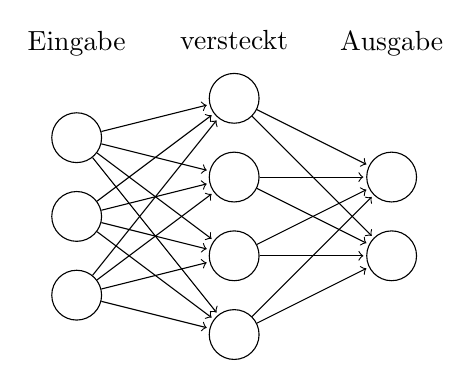
\begin{tikzpicture}
  \tikzstyle{node}=[circle,draw, minimum width=18pt, inner sep=0pt, fill=white]
  \tikzstyle{edge}=[->, shorten >= 1pt]

  \node[rectangle, inner sep=0pt] at (-2, 2.2) {Eingabe};
  \node[rectangle, inner sep=1pt] at (0,  2.24) {versteckt};
  \node[rectangle, inner sep=0pt] at (2,  2.2) {Ausgabe};

  \node[node] (a1) at (-2, -1) {};
  \node[node] (a2) at (-2, 0)  {};
  \node[node] (a3) at (-2, 1)  {};

  \node[node] (b1) at (0, -1.5) {};
  \node[node] (b2) at (0, -0.5) {};
  \node[node] (b3) at (0, 0.5)  {};
  \node[node] (b4) at (0, 1.5)  {};

  \node[node] (c1) at (2, -0.5) {};
  \node[node] (c2) at (2, 0.5)  {};

  \path[edge] (a1) edge (b1);
  \path[edge] (a1) edge (b2);
  \path[edge] (a1) edge (b3);
  \path[edge] (a1) edge (b4);
  \path[edge] (a2) edge (b1);
  \path[edge] (a2) edge (b2);
  \path[edge] (a2) edge (b3);
  \path[edge] (a2) edge (b4);
  \path[edge] (a3) edge (b1);
  \path[edge] (a3) edge (b2);
  \path[edge] (a3) edge (b3);
  \path[edge] (a3) edge (b4);
  \path[edge] (b1) edge (c1);
  \path[edge] (b1) edge (c2);
  \path[edge] (b2) edge (c1);
  \path[edge] (b2) edge (c2);
  \path[edge] (b3) edge (c1);
  \path[edge] (b3) edge (c2);
  \path[edge] (b4) edge (c1);
  \path[edge] (b4) edge (c2);
\end{tikzpicture}
\caption[Feedforward-Netz]{Beispiel eines Feedforward-Netzes mit drei vollverbundenen Schichten von einer Eingabe mit drei Neuronen zu einer Ausgabe mit zwei Neuronen und einer dazwischenliegenden versteckten Schicht.}
\label{fig:feedforward}
\end{figure}

Andere Netzvarianten erlauben \zB{} Schleifen, Rückwärtskanten oder das Überspringen einer Schicht~\cite{Nielsen}.

Ein Neuron besitzt genau einen reellen Wert, der sich aus den Neuronen der vorherigen Schicht erschließt.
Die $t$-te Neuronenschicht lässt sich folglich als ein Vektor $\ve{x}^{\left(t\right)} \in \gls{R}^{N^{\left(t\right)}}$ auffassen, wobei $N^{\left(t\right)} \in \gls{N}$ die Anzahl der Neuronen in der $t$-ten Schicht beschreibt.
Zu jeder Kante existiert zusätzlich ein Gewicht, welches den Anteil des Neurons zu dessen verbundenen Neuron angibt.
Damit lassen sich die Neuronenwerte der $\left(t+1\right)$-ten Schicht über
\begin{equation*}
  \ve{x}^{\left(t+1\right)} \coloneqq \gls{W}^{\left(t+1\right)}\ve{x}^{\left(t\right)}
\end{equation*}
definieren, wobei $\gls{W}^{\left(t+1\right)} \in \gls{R}^{N^{\left(t+1\right)} \times N^{\left(t\right)}}$ eine \emph{Gewichtsmatrix} der Kanten beschreibt, sodass $\gls{W}^{\left(t+1\right)}_{ji} \in \gls{R}$ das Gewicht der Kante des $i$-ten Neurons in der $t$-ten Schicht zu dem $j$-ten Neuron der $\left(t+1\right)$-ten Schicht angibt.
Zusätzlich zu den Gewichten existert zu jedem Neuron in der $t$-ten Schicht außer der Eingabeschicht ein \emph{Bias} $\gls{b}^{\left(t\right)} \in \gls{R}^{N^{\left(t\right)}}$.
Mit einer elementweisen Anwendung einer nicht-linearen \emph{Aktivierungsfunktion} $\gls{act} \colon \gls{R} \to \gls{R}$ ergibt sich damit die finale Version der Neuronenwerte der $\left(t+1\right)$-ten Schicht als
\begin{equation*}
  \ve{x}^{\left(t+1\right)} \coloneqq \gls{act} \left(\gls{W}^{\left(t+1\right)}\ve{x}^{\left(t\right)} + \gls{b}^{\left(t+1\right)} \right).
\end{equation*}
Als Aktivierungsfunktion kommt dabei \bspw{} die nicht-lineare \emph{Sigmoidfunktion} $\mathrm{sig}\left(z\right) \coloneqq 1 / \left(1 + \exp\left(-z\right)\right)$ oder die \emph{Rectified Linear Unit (ReLU)}-Funktion $\gls{relu}\left(z\right) \coloneqq \max \left(z, 0\right)$ zum Einsatz~\cite{Nielsen}.
Die Menge der Gewichte $\mathcal{W} \coloneqq {\left\{\gls{W}^{\left(t\right)}\right\}}_{t=2}^T$ sowie die Menge der Biaswerte $\mathcal{B} \coloneqq {\left\{\gls{b}^{\left(t\right)}\right\}}_{t=2}^T$ der $T \in \gls{N}$ vielen Schichten werden die \emph{Parameter} des Netzes genannt, über dessen Anpassung das Netz trainiert wird.
Diese Werte werden dabei sequentiell über einer kleinen Eingabemenge $\mathcal{X}$ mit den Eingaben $\ve{x} \in \mathcal{X}$ so angepasst, dass eine \emph{Kostenfunktion} minimiert wird.
Die Größe der Menge $\mathcal{X}$ wird dabei als \emph{Batch-Size} betitelt~\cite{Nielsen}.
Ein Beispiel einer Kostenfunktion ist die \emph{quadratische Kostenfunktion}, die über
\begin{equation}
  C\left(\mathcal{X}, \mathcal{W}, \mathcal{B}\right) \coloneqq \frac{1}{2\left|\mathcal{X}\right|} \sum_{\ve{x} \in \mathcal{X}} {\left\| \ve{y} - \ve{y}^{\prime} \right\|}_2^2
  \label{eq:quadratische_kostenfunktion}
\end{equation}
definiert ist, wobei \ve{y} die Ausgabe des Netzes und $\ve{y}^{\prime}$ die erwartete Ausgabe \bzgl{} \ve{x} beschreibt~\cite{Nielsen}.
Die implizit durch das Netz gegebenen Werte $\mathcal{W}$ und $\mathcal{B}$ werden dabei oft weggelassen, sodass wir lediglich $C\left(\mathcal{X}\right)$ schreiben.
$C$ zeichnet sich dabei als Kostenfunktion aus, denn sie ist für alle Eingaben stets positiv und wird umso kleiner, je ähnlicher \ve{y} und $\ve{y}^{\prime}$ werden.
Die Anpassung der Parameter des Netzes erfolgt über die sukzessive Eingabe einer Menge $\mathcal{X}$ in das Netz und der Berechnung eines negativen Gradienten in Richtung des steilsten Abstieges von $C$.
Formal betrachtet entspricht der Gradient der Kostenfunktion $C$ dem Vektor der partiellen Ableitungen
\begin{equation*}
  \nabla C \coloneqq {\left[\frac{\partial C}{\partial w_i}, \ldots, \frac{\partial C}{\partial b_j}, \ldots \right]}^{\top}
\end{equation*}
aller Gewichte $w_i$ und aller Biaswerte $b_j$ des Netzes~\cite{Nielsen}.
Durch die Anpassung der Gewichte und Biaswerte des Netzes über
\begin{equation*}
  w_i \rightarrow w^{\prime}_i = w_i - \gls{learning}\frac{\partial C}{\partial w_i}
  \qquad
  \text{und}
  \qquad
  b_j \rightarrow b^{\prime}_j = b_j - \gls{learning}\frac{\partial C}{\partial b_j}
\end{equation*}
wird die Kostenfunktion $C$ minimiert, wobei $\gls{learning} \in \gls{R+}$ der \emph{Lernrate}, \dhe{} der gewählten Schrittweite, entlang des negativen Gradienten entspricht~\cite{Nielsen}.
Üblicherweise wird dabei \gls{learning} so gewählt, dass das Netz nicht zu langsam trainiert, aber dennoch eine gute Approximation erreicht wird und erfordert in der Regel eine manuelle Anpassung.
Die Berechnung des Gradienten $\nabla C$ wird dabei aus Berechnungsgründen nicht für alle, sondern lediglich für Eingaben einer zufällig ausgewählten Untermenge von $\mathcal{X}$ durchgeführt und daraus dessen Durchschnitt gebildet, welcher stochastisch gesehen in etwa dem realen Gradienten über allen Eingaben entspricht (\emph{stochastischer Gradientenabstieg})~\cite{Nielsen}.
Zur Berechnung des Gradienten der Kostenfunktion $C$ kommt dabei der effiziente \emph{Backpropagation}-Algorithmus zum Einsatz, der es ermöglicht die optimierten Werte der Parameter nach einem Trainingsschritt zu ermitteln, indem der Fehler zwischen der Ausgabe des Netzes und der erwarteten Ausgabe über die Ausgabe- zur Eingabeschicht zurück propagiert wird~\cite{backpropagation}.
Aus den Fehlern der einzelnen Neuronen kann damit schließlich der Gradient $\nabla C$ berechnet werden (\vgl{}~\cite{Nielsen}).

Der Prozess des Trainings eines neuronalen Netzes, \dhe{} die Anpassung seiner Parameter zur Minimierung der Kostenfunktion, wird dabei solange wiederholt, bis $\nabla C$ ein lokales Minimum erreicht.
Ein einmaliges Durchlaufen aller Eingaben der Eingabemenge wird dabei als \emph{Epoche} bezeichnet~\cite{Nielsen}.
\\\\
Eine Spezialform eines neuronalen Netz ist das \emph{\gls{CNN}}, welches hauptsächlich in der Bild- und Spracherkennung zum Einsatz kommt und seinen Namen aufgrund der \emph{Faltung} seiner Eingabe mit einem \emph{Filter} erhält.~\cite{cnn}.
Entgegen eines Feedforward-Netzes, welches stets einen Vektor als Eingabe erwartet, arbeitet ein \gls{CNN} auf den originalen Bilddaten, \dhe{} einer Menge zweidimensionaler Matrizen, und ermöglicht so, dass dessen räumliche Struktur beim Lernen berücksichtigt wird~\cite{Nielsen}.
Dabei wird ein Neuron nicht mehr mit allen Neuronen der vorherigen Schicht, sondern nur noch mit einer Teilmenge dieser innerhalb eines Fensters um das Neuron verbunden.
Dieses Fenster wird auch oft, angelehnt an die Rezeptoren eines Auges, \emph{rezeptives Feld} (\engl{} \emph{Receptive-Field}) genannt~\cite{cnn}.
Die Größe des Receptive-Fields, \zB{} $5 \times 5$, wird dabei als \emph{Filtergröße} bezeichnet.
Abbildung~\ref{fig:cnn} veranschaulicht die Vernetzung der Neuronen durch ein Receptive-Field.
\section{Convolutional Neural Networks}
\label{convolutional_neural_networks}

Neuronale Netze \bzw{} Deep-Learning gehören zu den derzeit besten und beliebtesten Lösungen zu Problemen der Bild- oder Spracherkennung~\cite{Nielsen}.
Dabei lernt \bzw{} approximiert das Netz durch eine Anpassung ihrer Parameter über einer Menge an Trainingsbeispielen eine Funktion, sodass die Trainingsbeispiele auf ihre gewünschte Ausgabe abbilden und auch für unbekannte Eingaben zuverlässige Vorhersagen getroffen werden können.
Neuronale Netze sind daher größtenteils in dem Bereich des \emph{überwachten maschinellen Lernens} anzuordnen.
Ein Netz, welches lediglich die Trainingsmenge lernt, aber über der Trainingsmenge hinausgehende Daten nicht beschreiben kann, wird als ein \emph{überangepasstes} (\engl{} \emph{overfitted}) Netz bezeichnet~\cite{Nielsen}.

Ein \emph{neuronales Netz} besteht aus einer beliebigen Anzahl miteinander verbundener \emph{Neuronen}.
Neuronen sind üblicherweise mit anderen Neuronen in sequentiellen \emph{Schichten} \bzw{} \emph{Ebenen} angeordnet.
Die erste Schicht eines neuronalen Netzes wird als \emph{Eingabe}- und die letzte Schicht als  \emph{Ausgabeschicht} bezeichnet.
Schichten zwischen Ein- und Ausgabe heißen \emph{versteckt} (\engl{} \emph{hidden}).
Als \emph{Deep-Learning} wird ein Netz mit mindestens zwei versteckten Schichten verstanden.
Die einfachste Form eines neuronalen Netzes ist das \emph{Feedforward}-Netz, bei der jedes Neuron einer Schicht mit allen Neuronen der darauffolgenden Schicht verbunden ist.
Die Schichten eines Feedforward-Netzes werden deshalb auch als \emph{vollverbunden} (\engl{} \emph{fully-connected}) betitelt.
Abbildung~\ref{fig:feedforward} zeigt ein Beispiel eines solchen Netzes mit drei Schichten.
\begin{figure}[t]
\centering
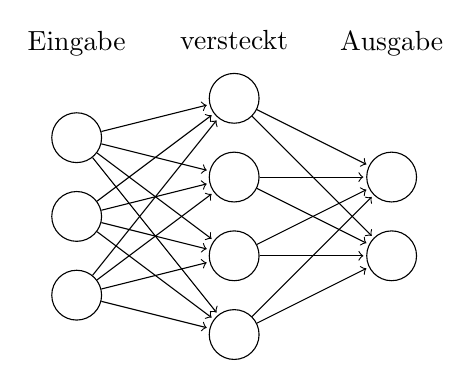
\begin{tikzpicture}
  \tikzstyle{node}=[circle,draw, minimum width=18pt, inner sep=0pt, fill=white]
  \tikzstyle{edge}=[->, shorten >= 1pt]

  \node[rectangle, inner sep=0pt] at (-2, 2.2) {Eingabe};
  \node[rectangle, inner sep=1pt] at (0,  2.24) {versteckt};
  \node[rectangle, inner sep=0pt] at (2,  2.2) {Ausgabe};

  \node[node] (a1) at (-2, -1) {};
  \node[node] (a2) at (-2, 0)  {};
  \node[node] (a3) at (-2, 1)  {};

  \node[node] (b1) at (0, -1.5) {};
  \node[node] (b2) at (0, -0.5) {};
  \node[node] (b3) at (0, 0.5)  {};
  \node[node] (b4) at (0, 1.5)  {};

  \node[node] (c1) at (2, -0.5) {};
  \node[node] (c2) at (2, 0.5)  {};

  \path[edge] (a1) edge (b1);
  \path[edge] (a1) edge (b2);
  \path[edge] (a1) edge (b3);
  \path[edge] (a1) edge (b4);
  \path[edge] (a2) edge (b1);
  \path[edge] (a2) edge (b2);
  \path[edge] (a2) edge (b3);
  \path[edge] (a2) edge (b4);
  \path[edge] (a3) edge (b1);
  \path[edge] (a3) edge (b2);
  \path[edge] (a3) edge (b3);
  \path[edge] (a3) edge (b4);
  \path[edge] (b1) edge (c1);
  \path[edge] (b1) edge (c2);
  \path[edge] (b2) edge (c1);
  \path[edge] (b2) edge (c2);
  \path[edge] (b3) edge (c1);
  \path[edge] (b3) edge (c2);
  \path[edge] (b4) edge (c1);
  \path[edge] (b4) edge (c2);
\end{tikzpicture}
\caption[Feedforward-Netz]{Beispiel eines Feedforward-Netzes mit drei vollverbundenen Schichten von einer Eingabe mit drei Neuronen zu einer Ausgabe mit zwei Neuronen und einer dazwischenliegenden versteckten Schicht.}
\label{fig:feedforward}
\end{figure}

Andere Netzvarianten erlauben \zB{} Schleifen, Rückwärtskanten oder das Überspringen einer Schicht~\cite{Nielsen}.

Ein Neuron besitzt genau einen reellen Wert, der sich aus den Neuronen der vorherigen Schicht erschließt.
Die $t$-te Neuronenschicht lässt sich folglich als ein Vektor $\ve{x}^{\left(t\right)} \in \gls{R}^{N^{\left(t\right)}}$ auffassen, wobei $N^{\left(t\right)} \in \gls{N}$ die Anzahl der Neuronen in der $t$-ten Schicht beschreibt.
Zu jeder Kante existiert zusätzlich ein Gewicht, welches den Anteil des Neurons zu dessen verbundenen Neuron angibt.
Damit lassen sich die Neuronenwerte der $\left(t+1\right)$-ten Schicht über
\begin{equation*}
  \ve{x}^{\left(t+1\right)} \coloneqq \gls{W}^{\left(t+1\right)}\ve{x}^{\left(t\right)}
\end{equation*}
definieren, wobei $\gls{W}^{\left(t+1\right)} \in \gls{R}^{N^{\left(t+1\right)} \times N^{\left(t\right)}}$ eine \emph{Gewichtsmatrix} der Kanten beschreibt, sodass $\gls{W}^{\left(t+1\right)}_{ji} \in \gls{R}$ das Gewicht der Kante des $i$-ten Neurons in der $t$-ten Schicht zu dem $j$-ten Neuron der $\left(t+1\right)$-ten Schicht angibt.
Zusätzlich zu den Gewichten existert zu jedem Neuron in der $t$-ten Schicht außer der Eingabeschicht ein \emph{Bias} $\gls{b}^{\left(t\right)} \in \gls{R}^{N^{\left(t\right)}}$.
Mit einer elementweisen Anwendung einer nicht-linearen \emph{Aktivierungsfunktion} $\gls{act} \colon \gls{R} \to \gls{R}$ ergibt sich damit die finale Version der Neuronenwerte der $\left(t+1\right)$-ten Schicht als
\begin{equation*}
  \ve{x}^{\left(t+1\right)} \coloneqq \gls{act} \left(\gls{W}^{\left(t+1\right)}\ve{x}^{\left(t\right)} + \gls{b}^{\left(t+1\right)} \right).
\end{equation*}
Als Aktivierungsfunktion kommt dabei \bspw{} die nicht-lineare \emph{Sigmoidfunktion} $\mathrm{sig}\left(z\right) \coloneqq 1 / \left(1 + \exp\left(-z\right)\right)$ oder die \emph{Rectified Linear Unit (ReLU)}-Funktion $\gls{relu}\left(z\right) \coloneqq \max \left(z, 0\right)$ zum Einsatz~\cite{Nielsen}.
Die Menge der Gewichte $\mathcal{W} \coloneqq {\left\{\gls{W}^{\left(t\right)}\right\}}_{t=2}^T$ sowie die Menge der Biaswerte $\mathcal{B} \coloneqq {\left\{\gls{b}^{\left(t\right)}\right\}}_{t=2}^T$ der $T \in \gls{N}$ vielen Schichten werden die \emph{Parameter} des Netzes genannt, über dessen Anpassung das Netz trainiert wird.
Diese Werte werden dabei sequentiell über einer kleinen Eingabemenge $\mathcal{X}$ mit den Eingaben $\ve{x} \in \mathcal{X}$ so angepasst, dass eine \emph{Kostenfunktion} minimiert wird.
Die Größe der Menge $\mathcal{X}$ wird dabei als \emph{Batch-Size} betitelt~\cite{Nielsen}.
Ein Beispiel einer Kostenfunktion ist die \emph{quadratische Kostenfunktion}, die über
\begin{equation}
  C\left(\mathcal{X}, \mathcal{W}, \mathcal{B}\right) \coloneqq \frac{1}{2\left|\mathcal{X}\right|} \sum_{\ve{x} \in \mathcal{X}} {\left\| \ve{y} - \ve{y}^{\prime} \right\|}_2^2
  \label{eq:quadratische_kostenfunktion}
\end{equation}
definiert ist, wobei \ve{y} die Ausgabe des Netzes und $\ve{y}^{\prime}$ die erwartete Ausgabe \bzgl{} \ve{x} beschreibt~\cite{Nielsen}.
Die implizit durch das Netz gegebenen Werte $\mathcal{W}$ und $\mathcal{B}$ werden dabei oft weggelassen, sodass wir lediglich $C\left(\mathcal{X}\right)$ schreiben.
$C$ zeichnet sich dabei als Kostenfunktion aus, denn sie ist für alle Eingaben stets positiv und wird umso kleiner, je ähnlicher \ve{y} und $\ve{y}^{\prime}$ werden.
Die Anpassung der Parameter des Netzes erfolgt über die sukzessive Eingabe einer Menge $\mathcal{X}$ in das Netz und der Berechnung eines negativen Gradienten in Richtung des steilsten Abstieges von $C$.
Formal betrachtet entspricht der Gradient der Kostenfunktion $C$ dem Vektor der partiellen Ableitungen
\begin{equation*}
  \nabla C \coloneqq {\left[\frac{\partial C}{\partial w_i}, \ldots, \frac{\partial C}{\partial b_j}, \ldots \right]}^{\top}
\end{equation*}
aller Gewichte $w_i$ und aller Biaswerte $b_j$ des Netzes~\cite{Nielsen}.
Durch die Anpassung der Gewichte und Biaswerte des Netzes über
\begin{equation*}
  w_i \rightarrow w^{\prime}_i = w_i - \gls{learning}\frac{\partial C}{\partial w_i}
  \qquad
  \text{und}
  \qquad
  b_j \rightarrow b^{\prime}_j = b_j - \gls{learning}\frac{\partial C}{\partial b_j}
\end{equation*}
wird die Kostenfunktion $C$ minimiert, wobei $\gls{learning} \in \gls{R+}$ der \emph{Lernrate}, \dhe{} der gewählten Schrittweite, entlang des negativen Gradienten entspricht~\cite{Nielsen}.
Üblicherweise wird dabei \gls{learning} so gewählt, dass das Netz nicht zu langsam trainiert, aber dennoch eine gute Approximation erreicht wird und erfordert in der Regel eine manuelle Anpassung.
Die Berechnung des Gradienten $\nabla C$ wird dabei aus Berechnungsgründen nicht für alle, sondern lediglich für Eingaben einer zufällig ausgewählten Untermenge von $\mathcal{X}$ durchgeführt und daraus dessen Durchschnitt gebildet, welcher stochastisch gesehen in etwa dem realen Gradienten über allen Eingaben entspricht (\emph{stochastischer Gradientenabstieg})~\cite{Nielsen}.
Zur Berechnung des Gradienten der Kostenfunktion $C$ kommt dabei der effiziente \emph{Backpropagation}-Algorithmus zum Einsatz, der es ermöglicht die optimierten Werte der Parameter nach einem Trainingsschritt zu ermitteln, indem der Fehler zwischen der Ausgabe des Netzes und der erwarteten Ausgabe über die Ausgabe- zur Eingabeschicht zurück propagiert wird~\cite{backpropagation}.
Aus den Fehlern der einzelnen Neuronen kann damit schließlich der Gradient $\nabla C$ berechnet werden (\vgl{}~\cite{Nielsen}).

Der Prozess des Trainings eines neuronalen Netzes, \dhe{} die Anpassung seiner Parameter zur Minimierung der Kostenfunktion, wird dabei solange wiederholt, bis $\nabla C$ ein lokales Minimum erreicht.
Ein einmaliges Durchlaufen aller Eingaben der Eingabemenge wird dabei als \emph{Epoche} bezeichnet~\cite{Nielsen}.
\\\\
Eine Spezialform eines neuronalen Netz ist das \emph{\gls{CNN}}, welches hauptsächlich in der Bild- und Spracherkennung zum Einsatz kommt und seinen Namen aufgrund der \emph{Faltung} seiner Eingabe mit einem \emph{Filter} erhält.~\cite{cnn}.
Entgegen eines Feedforward-Netzes, welches stets einen Vektor als Eingabe erwartet, arbeitet ein \gls{CNN} auf den originalen Bilddaten, \dhe{} einer Menge zweidimensionaler Matrizen, und ermöglicht so, dass dessen räumliche Struktur beim Lernen berücksichtigt wird~\cite{Nielsen}.
Dabei wird ein Neuron nicht mehr mit allen Neuronen der vorherigen Schicht, sondern nur noch mit einer Teilmenge dieser innerhalb eines Fensters um das Neuron verbunden.
Dieses Fenster wird auch oft, angelehnt an die Rezeptoren eines Auges, \emph{rezeptives Feld} (\engl{} \emph{Receptive-Field}) genannt~\cite{cnn}.
Die Größe des Receptive-Fields, \zB{} $5 \times 5$, wird dabei als \emph{Filtergröße} bezeichnet.
Abbildung~\ref{fig:cnn} veranschaulicht die Vernetzung der Neuronen durch ein Receptive-Field.
\section{Convolutional Neural Networks}
\label{convolutional_neural_networks}

Neuronale Netze \bzw{} Deep-Learning gehören zu den derzeit besten und beliebtesten Lösungen zu Problemen der Bild- oder Spracherkennung~\cite{Nielsen}.
Dabei lernt \bzw{} approximiert das Netz durch eine Anpassung ihrer Parameter über einer Menge an Trainingsbeispielen eine Funktion, sodass die Trainingsbeispiele auf ihre gewünschte Ausgabe abbilden und auch für unbekannte Eingaben zuverlässige Vorhersagen getroffen werden können.
Neuronale Netze sind daher größtenteils in dem Bereich des \emph{überwachten maschinellen Lernens} anzuordnen.
Ein Netz, welches lediglich die Trainingsmenge lernt, aber über der Trainingsmenge hinausgehende Daten nicht beschreiben kann, wird als ein \emph{überangepasstes} (\engl{} \emph{overfitted}) Netz bezeichnet~\cite{Nielsen}.

Ein \emph{neuronales Netz} besteht aus einer beliebigen Anzahl miteinander verbundener \emph{Neuronen}.
Neuronen sind üblicherweise mit anderen Neuronen in sequentiellen \emph{Schichten} \bzw{} \emph{Ebenen} angeordnet.
Die erste Schicht eines neuronalen Netzes wird als \emph{Eingabe}- und die letzte Schicht als  \emph{Ausgabeschicht} bezeichnet.
Schichten zwischen Ein- und Ausgabe heißen \emph{versteckt} (\engl{} \emph{hidden}).
Als \emph{Deep-Learning} wird ein Netz mit mindestens zwei versteckten Schichten verstanden.
Die einfachste Form eines neuronalen Netzes ist das \emph{Feedforward}-Netz, bei der jedes Neuron einer Schicht mit allen Neuronen der darauffolgenden Schicht verbunden ist.
Die Schichten eines Feedforward-Netzes werden deshalb auch als \emph{vollverbunden} (\engl{} \emph{fully-connected}) betitelt.
Abbildung~\ref{fig:feedforward} zeigt ein Beispiel eines solchen Netzes mit drei Schichten.
\input{tikz/feedforward}
Andere Netzvarianten erlauben \zB{} Schleifen, Rückwärtskanten oder das Überspringen einer Schicht~\cite{Nielsen}.

Ein Neuron besitzt genau einen reellen Wert, der sich aus den Neuronen der vorherigen Schicht erschließt.
Die $t$-te Neuronenschicht lässt sich folglich als ein Vektor $\ve{x}^{\left(t\right)} \in \gls{R}^{N^{\left(t\right)}}$ auffassen, wobei $N^{\left(t\right)} \in \gls{N}$ die Anzahl der Neuronen in der $t$-ten Schicht beschreibt.
Zu jeder Kante existiert zusätzlich ein Gewicht, welches den Anteil des Neurons zu dessen verbundenen Neuron angibt.
Damit lassen sich die Neuronenwerte der $\left(t+1\right)$-ten Schicht über
\begin{equation*}
  \ve{x}^{\left(t+1\right)} \coloneqq \gls{W}^{\left(t+1\right)}\ve{x}^{\left(t\right)}
\end{equation*}
definieren, wobei $\gls{W}^{\left(t+1\right)} \in \gls{R}^{N^{\left(t+1\right)} \times N^{\left(t\right)}}$ eine \emph{Gewichtsmatrix} der Kanten beschreibt, sodass $\gls{W}^{\left(t+1\right)}_{ji} \in \gls{R}$ das Gewicht der Kante des $i$-ten Neurons in der $t$-ten Schicht zu dem $j$-ten Neuron der $\left(t+1\right)$-ten Schicht angibt.
Zusätzlich zu den Gewichten existert zu jedem Neuron in der $t$-ten Schicht außer der Eingabeschicht ein \emph{Bias} $\gls{b}^{\left(t\right)} \in \gls{R}^{N^{\left(t\right)}}$.
Mit einer elementweisen Anwendung einer nicht-linearen \emph{Aktivierungsfunktion} $\gls{act} \colon \gls{R} \to \gls{R}$ ergibt sich damit die finale Version der Neuronenwerte der $\left(t+1\right)$-ten Schicht als
\begin{equation*}
  \ve{x}^{\left(t+1\right)} \coloneqq \gls{act} \left(\gls{W}^{\left(t+1\right)}\ve{x}^{\left(t\right)} + \gls{b}^{\left(t+1\right)} \right).
\end{equation*}
Als Aktivierungsfunktion kommt dabei \bspw{} die nicht-lineare \emph{Sigmoidfunktion} $\mathrm{sig}\left(z\right) \coloneqq 1 / \left(1 + \exp\left(-z\right)\right)$ oder die \emph{Rectified Linear Unit (ReLU)}-Funktion $\gls{relu}\left(z\right) \coloneqq \max \left(z, 0\right)$ zum Einsatz~\cite{Nielsen}.
Die Menge der Gewichte $\mathcal{W} \coloneqq {\left\{\gls{W}^{\left(t\right)}\right\}}_{t=2}^T$ sowie die Menge der Biaswerte $\mathcal{B} \coloneqq {\left\{\gls{b}^{\left(t\right)}\right\}}_{t=2}^T$ der $T \in \gls{N}$ vielen Schichten werden die \emph{Parameter} des Netzes genannt, über dessen Anpassung das Netz trainiert wird.
Diese Werte werden dabei sequentiell über einer kleinen Eingabemenge $\mathcal{X}$ mit den Eingaben $\ve{x} \in \mathcal{X}$ so angepasst, dass eine \emph{Kostenfunktion} minimiert wird.
Die Größe der Menge $\mathcal{X}$ wird dabei als \emph{Batch-Size} betitelt~\cite{Nielsen}.
Ein Beispiel einer Kostenfunktion ist die \emph{quadratische Kostenfunktion}, die über
\begin{equation}
  C\left(\mathcal{X}, \mathcal{W}, \mathcal{B}\right) \coloneqq \frac{1}{2\left|\mathcal{X}\right|} \sum_{\ve{x} \in \mathcal{X}} {\left\| \ve{y} - \ve{y}^{\prime} \right\|}_2^2
  \label{eq:quadratische_kostenfunktion}
\end{equation}
definiert ist, wobei \ve{y} die Ausgabe des Netzes und $\ve{y}^{\prime}$ die erwartete Ausgabe \bzgl{} \ve{x} beschreibt~\cite{Nielsen}.
Die implizit durch das Netz gegebenen Werte $\mathcal{W}$ und $\mathcal{B}$ werden dabei oft weggelassen, sodass wir lediglich $C\left(\mathcal{X}\right)$ schreiben.
$C$ zeichnet sich dabei als Kostenfunktion aus, denn sie ist für alle Eingaben stets positiv und wird umso kleiner, je ähnlicher \ve{y} und $\ve{y}^{\prime}$ werden.
Die Anpassung der Parameter des Netzes erfolgt über die sukzessive Eingabe einer Menge $\mathcal{X}$ in das Netz und der Berechnung eines negativen Gradienten in Richtung des steilsten Abstieges von $C$.
Formal betrachtet entspricht der Gradient der Kostenfunktion $C$ dem Vektor der partiellen Ableitungen
\begin{equation*}
  \nabla C \coloneqq {\left[\frac{\partial C}{\partial w_i}, \ldots, \frac{\partial C}{\partial b_j}, \ldots \right]}^{\top}
\end{equation*}
aller Gewichte $w_i$ und aller Biaswerte $b_j$ des Netzes~\cite{Nielsen}.
Durch die Anpassung der Gewichte und Biaswerte des Netzes über
\begin{equation*}
  w_i \rightarrow w^{\prime}_i = w_i - \gls{learning}\frac{\partial C}{\partial w_i}
  \qquad
  \text{und}
  \qquad
  b_j \rightarrow b^{\prime}_j = b_j - \gls{learning}\frac{\partial C}{\partial b_j}
\end{equation*}
wird die Kostenfunktion $C$ minimiert, wobei $\gls{learning} \in \gls{R+}$ der \emph{Lernrate}, \dhe{} der gewählten Schrittweite, entlang des negativen Gradienten entspricht~\cite{Nielsen}.
Üblicherweise wird dabei \gls{learning} so gewählt, dass das Netz nicht zu langsam trainiert, aber dennoch eine gute Approximation erreicht wird und erfordert in der Regel eine manuelle Anpassung.
Die Berechnung des Gradienten $\nabla C$ wird dabei aus Berechnungsgründen nicht für alle, sondern lediglich für Eingaben einer zufällig ausgewählten Untermenge von $\mathcal{X}$ durchgeführt und daraus dessen Durchschnitt gebildet, welcher stochastisch gesehen in etwa dem realen Gradienten über allen Eingaben entspricht (\emph{stochastischer Gradientenabstieg})~\cite{Nielsen}.
Zur Berechnung des Gradienten der Kostenfunktion $C$ kommt dabei der effiziente \emph{Backpropagation}-Algorithmus zum Einsatz, der es ermöglicht die optimierten Werte der Parameter nach einem Trainingsschritt zu ermitteln, indem der Fehler zwischen der Ausgabe des Netzes und der erwarteten Ausgabe über die Ausgabe- zur Eingabeschicht zurück propagiert wird~\cite{backpropagation}.
Aus den Fehlern der einzelnen Neuronen kann damit schließlich der Gradient $\nabla C$ berechnet werden (\vgl{}~\cite{Nielsen}).

Der Prozess des Trainings eines neuronalen Netzes, \dhe{} die Anpassung seiner Parameter zur Minimierung der Kostenfunktion, wird dabei solange wiederholt, bis $\nabla C$ ein lokales Minimum erreicht.
Ein einmaliges Durchlaufen aller Eingaben der Eingabemenge wird dabei als \emph{Epoche} bezeichnet~\cite{Nielsen}.
\\\\
Eine Spezialform eines neuronalen Netz ist das \emph{\gls{CNN}}, welches hauptsächlich in der Bild- und Spracherkennung zum Einsatz kommt und seinen Namen aufgrund der \emph{Faltung} seiner Eingabe mit einem \emph{Filter} erhält.~\cite{cnn}.
Entgegen eines Feedforward-Netzes, welches stets einen Vektor als Eingabe erwartet, arbeitet ein \gls{CNN} auf den originalen Bilddaten, \dhe{} einer Menge zweidimensionaler Matrizen, und ermöglicht so, dass dessen räumliche Struktur beim Lernen berücksichtigt wird~\cite{Nielsen}.
Dabei wird ein Neuron nicht mehr mit allen Neuronen der vorherigen Schicht, sondern nur noch mit einer Teilmenge dieser innerhalb eines Fensters um das Neuron verbunden.
Dieses Fenster wird auch oft, angelehnt an die Rezeptoren eines Auges, \emph{rezeptives Feld} (\engl{} \emph{Receptive-Field}) genannt~\cite{cnn}.
Die Größe des Receptive-Fields, \zB{} $5 \times 5$, wird dabei als \emph{Filtergröße} bezeichnet.
Abbildung~\ref{fig:cnn} veranschaulicht die Vernetzung der Neuronen durch ein Receptive-Field.
\input{tikz/cnn}
Eine Besonderheit des \glspl{CNN} ist weiterhin, dass sich die Receptive-Fields ihre Gewichte und Biaswerte teilen.
Damit erlernt ein Receptive-Field ein Merkmal, \zB{} eine Kante oder eine Textur, und findet dieses Merkmal auch in anderen Receptive-Fields, nur an unterschiedlichen Positionen~\cite{Nielsen}.
Das ermöglicht insbesondere das Erlernen translationsinvarianter Merkmale, die für eine Bilderkennung fundamental sind.
Aus diesem Grund spricht man auch häufig von einer \emph{Merkmalskarte} (\engl{} \emph{Feature-Map}), die durch eine Faltung über den Receptive-Fields entsteht.
Um mehrere Merkmale eines Receptive-Fields zu generieren, werden dabei üblicherweise eine Reihe von zusammengehörigen \emph{Eingabekarten} auf eine neue Menge von \emph{Ausgabekarten} projiziert.
Ein Bild $\gls{B} \in \gls{R}^{H \times W \times 3}$ mit drei Farbkanälen beschreibt \zB{} drei Merkmalskarten, die als Eingabe in das \gls{CNN} dienen.

Formal lässt sich damit die \emph{zweidimensionale Faltungsoperation}
\begin{equation*}
  \gls{conv2d} \gls{R}^{\colon H \times W \times M_{\mathrm{in}}} \to \gls{R}^{H \times W \times M_{\mathrm{out}}},
\end{equation*}
im Folgenden auch oft als \emph{klassische Faltungsoperation} betitelt, als
\begin{equation*}
  {\gls{conv2d}\left(\gls{B}\right)}_{yxm} \coloneqq \sum_{\Delta y = 1}^{F_y} \sum_{\Delta x = 1}^{F_x} \sum_{m_{\mathrm{in}} = 1}^{M_\mathrm{in}} \gls{B}_{y + \left\lceil F_y/2 \right\rceil - \Delta y, x + \left\lceil F_x/2 \right\rceil - \Delta x, m_{\mathrm{in}}} \gls{W}_{\Delta y, \Delta x, m_{\mathrm{in}}, m}
\end{equation*}
mit $1 \leq y \leq H$, $1 \leq x \leq W$ und $1 \leq m \leq M_{\mathrm{out}}$ definieren, wobei $\gls{B} \in \gls{R}^{H \times W \times M_{\mathrm{in}}}$ die Eingabe und $\gls{W} \in \gls{R}^{F_y \times F_x \times M_{\mathrm{in}} \times M_{\mathrm{out}}}$ den Filter \bzw{} Gewichtstensor der Faltungsoperation mit Filtergröße $F_y \times F_x$ von $M_{\mathrm{in}} \in \gls{N}$ Eingabekarten auf $M_{\mathrm{out}} \in \gls{N}$ Ausgabekarten beschreibt~\cite{tensorflow}.
Auf die Aufsummierung eines Bias $\gls{b} \in \gls{R}^{M_{\mathrm{out}}}$ sowie die Anwendung der Aktivierungsfunktion \gls{act} auf \gls{conv2d} wurde hier zur Vereinfachung verzichtet.
Der Wert eines Indexzugriffs auf die Eingabekarte \gls{B}, der über die Grenzen von \gls{B} hinausgeht, wird üblicherweise auf Null gesetzt (\emph{Zero-Padding}), sodass dieser keinen Einfluss auf die Faltung nimmt und die Ausgabekarte damit die gleiche Höhe und Breite der Eingabekarte besitzt~\cite{tensorflow}.
Eine Reduktion der Auflösung innerhalb der Faltungsschicht kann erreicht werden, indem nicht über jedes Neuron, sondern nur über eine Untermenge dieser in fester Schrittweite $s_y \times s_x$ zueinander gefaltet wird.
Eine Alternative dazu ist die Verwendung einer \emph{Poo\-ling\-sch\-icht}, die üblicherweise direkt nach einer Faltungsschicht zum Einsatz kommt und versucht, die Ausgabe der Faltungsschicht zu reduzieren \bzw{} auf das Wesentliche zu vereinfachen.
Eine Poolingoperation besitzt analog zu \gls{conv2d} eine Fenstergröße sowie eine Schrittweite.
Die beliebteste Poolingoperation ist das \emph{Max-Pooling}, welche sich jeweils für das Maximum der Aktivierungen innerhalb jedes Fensters entscheidet~\cite{Nielsen}.
Eine Poolingoperation mit Fenstergröße $2 \times 2$ sowie Schrittweite $2 \times 2$ reduziert damit die Daten der Merkmalskarte um genau die Hälfte.

Ein \gls{CNN} besteht typischerweise aus mehreren Faltungs- und Poolingschichten, sodass die Menge der Merkmalskarten dabei stetig erhöht und die Auflösung stetig verringert wird~\cite{Nielsen}.
Damit entstehen im späteren Verlauf des Netzes Merkmalskarten, die immer größere Receptive-Fields des Eingabebildes basierend auf den ermittelten Merkmalen vorangegangener Schichten beschreiben.
Nach einer gewissen Anzahl an Faltungen werden die Merkmalskarten zu einem Vektor umsortiert, sodass vollverbundene Schichten hin zur Ausgabe genutzt werden können~\cite{Nielsen}.
Abbildung~\ref{fig:cnn_aufbau} illustriert den üblichen Aufbau eines \glspl{CNN}.
\input{tikz/cnn_aufbau}

Eine Besonderheit des \glspl{CNN} ist weiterhin, dass sich die Receptive-Fields ihre Gewichte und Biaswerte teilen.
Damit erlernt ein Receptive-Field ein Merkmal, \zB{} eine Kante oder eine Textur, und findet dieses Merkmal auch in anderen Receptive-Fields, nur an unterschiedlichen Positionen~\cite{Nielsen}.
Das ermöglicht insbesondere das Erlernen translationsinvarianter Merkmale, die für eine Bilderkennung fundamental sind.
Aus diesem Grund spricht man auch häufig von einer \emph{Merkmalskarte} (\engl{} \emph{Feature-Map}), die durch eine Faltung über den Receptive-Fields entsteht.
Um mehrere Merkmale eines Receptive-Fields zu generieren, werden dabei üblicherweise eine Reihe von zusammengehörigen \emph{Eingabekarten} auf eine neue Menge von \emph{Ausgabekarten} projiziert.
Ein Bild $\gls{B} \in \gls{R}^{H \times W \times 3}$ mit drei Farbkanälen beschreibt \zB{} drei Merkmalskarten, die als Eingabe in das \gls{CNN} dienen.

Formal lässt sich damit die \emph{zweidimensionale Faltungsoperation}
\begin{equation*}
  \gls{conv2d} \gls{R}^{\colon H \times W \times M_{\mathrm{in}}} \to \gls{R}^{H \times W \times M_{\mathrm{out}}},
\end{equation*}
im Folgenden auch oft als \emph{klassische Faltungsoperation} betitelt, als
\begin{equation*}
  {\gls{conv2d}\left(\gls{B}\right)}_{yxm} \coloneqq \sum_{\Delta y = 1}^{F_y} \sum_{\Delta x = 1}^{F_x} \sum_{m_{\mathrm{in}} = 1}^{M_\mathrm{in}} \gls{B}_{y + \left\lceil F_y/2 \right\rceil - \Delta y, x + \left\lceil F_x/2 \right\rceil - \Delta x, m_{\mathrm{in}}} \gls{W}_{\Delta y, \Delta x, m_{\mathrm{in}}, m}
\end{equation*}
mit $1 \leq y \leq H$, $1 \leq x \leq W$ und $1 \leq m \leq M_{\mathrm{out}}$ definieren, wobei $\gls{B} \in \gls{R}^{H \times W \times M_{\mathrm{in}}}$ die Eingabe und $\gls{W} \in \gls{R}^{F_y \times F_x \times M_{\mathrm{in}} \times M_{\mathrm{out}}}$ den Filter \bzw{} Gewichtstensor der Faltungsoperation mit Filtergröße $F_y \times F_x$ von $M_{\mathrm{in}} \in \gls{N}$ Eingabekarten auf $M_{\mathrm{out}} \in \gls{N}$ Ausgabekarten beschreibt~\cite{tensorflow}.
Auf die Aufsummierung eines Bias $\gls{b} \in \gls{R}^{M_{\mathrm{out}}}$ sowie die Anwendung der Aktivierungsfunktion \gls{act} auf \gls{conv2d} wurde hier zur Vereinfachung verzichtet.
Der Wert eines Indexzugriffs auf die Eingabekarte \gls{B}, der über die Grenzen von \gls{B} hinausgeht, wird üblicherweise auf Null gesetzt (\emph{Zero-Padding}), sodass dieser keinen Einfluss auf die Faltung nimmt und die Ausgabekarte damit die gleiche Höhe und Breite der Eingabekarte besitzt~\cite{tensorflow}.
Eine Reduktion der Auflösung innerhalb der Faltungsschicht kann erreicht werden, indem nicht über jedes Neuron, sondern nur über eine Untermenge dieser in fester Schrittweite $s_y \times s_x$ zueinander gefaltet wird.
Eine Alternative dazu ist die Verwendung einer \emph{Poo\-ling\-sch\-icht}, die üblicherweise direkt nach einer Faltungsschicht zum Einsatz kommt und versucht, die Ausgabe der Faltungsschicht zu reduzieren \bzw{} auf das Wesentliche zu vereinfachen.
Eine Poolingoperation besitzt analog zu \gls{conv2d} eine Fenstergröße sowie eine Schrittweite.
Die beliebteste Poolingoperation ist das \emph{Max-Pooling}, welche sich jeweils für das Maximum der Aktivierungen innerhalb jedes Fensters entscheidet~\cite{Nielsen}.
Eine Poolingoperation mit Fenstergröße $2 \times 2$ sowie Schrittweite $2 \times 2$ reduziert damit die Daten der Merkmalskarte um genau die Hälfte.

Ein \gls{CNN} besteht typischerweise aus mehreren Faltungs- und Poolingschichten, sodass die Menge der Merkmalskarten dabei stetig erhöht und die Auflösung stetig verringert wird~\cite{Nielsen}.
Damit entstehen im späteren Verlauf des Netzes Merkmalskarten, die immer größere Receptive-Fields des Eingabebildes basierend auf den ermittelten Merkmalen vorangegangener Schichten beschreiben.
Nach einer gewissen Anzahl an Faltungen werden die Merkmalskarten zu einem Vektor umsortiert, sodass vollverbundene Schichten hin zur Ausgabe genutzt werden können~\cite{Nielsen}.
Abbildung~\ref{fig:cnn_aufbau} illustriert den üblichen Aufbau eines \glspl{CNN}.
\begin{figure}[t]
\centering
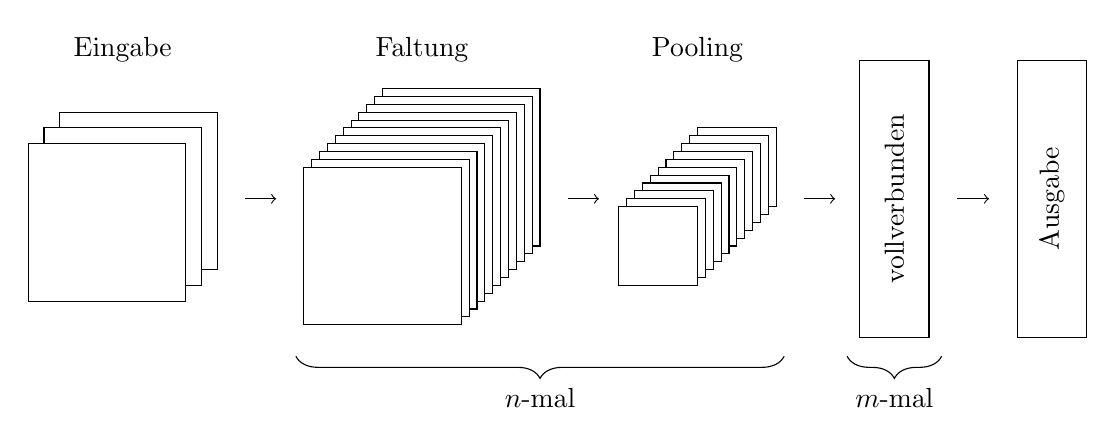
\begin{tikzpicture}
  \tikzstyle{node}=[rectangle, draw, minimum width=100pt, minimum height=25pt, inner sep=0pt, fill=white, rotate=90]
  \tikzstyle{rect}=[rectangle, draw, fill=white]
  \tikzstyle{path}=[->, shorten >= 10pt, shorten <= 10pt]

  % Eingabe.
  \draw[rect] (-0.1, 0.4) rectangle (1.9, 2.4);
  \draw[rect] (-0.3, 0.2) rectangle (1.7, 2.2);
  \draw[rect] (-0.5, 0)   rectangle (1.5, 2);

  % Faltung.
  \draw[rect] (4,   0.7)  rectangle (6,   2.7);
  \draw[rect] (3.9, 0.6)  rectangle (5.9, 2.6);
  \draw[rect] (3.8, 0.5)  rectangle (5.8, 2.5);
  \draw[rect] (3.7, 0.4)  rectangle (5.7, 2.4);
  \draw[rect] (3.6, 0.3)  rectangle (5.6, 2.3);
  \draw[rect] (3.5, 0.2)  rectangle (5.5, 2.2);
  \draw[rect] (3.4, 0.1)  rectangle (5.4, 2.1);
  \draw[rect] (3.3, 0)    rectangle (5.3, 2);
  \draw[rect] (3.2, -0.1) rectangle (5.2, 1.9);
  \draw[rect] (3.1, -0.2) rectangle (5.1, 1.8);
  \draw[rect] (3,   -0.3) rectangle (5, 1.7);

  % Pooling.
  \draw[rect] (8,   1.2) rectangle (9,   2.2);
  \draw[rect] (7.9, 1.1) rectangle (8.9, 2.1);
  \draw[rect] (7.8, 1)   rectangle (8.8, 2);
  \draw[rect] (7.7, 0.9) rectangle (8.7, 1.9);
  \draw[rect] (7.6, 0.8) rectangle (8.6, 1.8);
  \draw[rect] (7.5, 0.7) rectangle (8.5, 1.7);
  \draw[rect] (7.4, 0.6) rectangle (8.4, 1.6);
  \draw[rect] (7.3, 0.5) rectangle (8.3, 1.5);
  \draw[rect] (7.2, 0.4) rectangle (8.2, 1.4);
  \draw[rect] (7.1, 0.3) rectangle (8.1, 1.3);
  \draw[rect] (7,   0.2) rectangle (8,   1.2);

  \node at (0.7, 3.2) {Eingabe};
  \node at (4.5, 3.2) {Faltung};
  \node at (8,   3.2) {Pooling};

  \node[node] (1)  at (10.5, 1.3) {vollverbunden};
  \node[node] (2)  at (12.5, 1.3) {Ausgabe};

  \path[path] (1.9, 1.3) edge (3,    1.3);
  \path[path] (6, 1.3)   edge (7.1,  1.3);
  \path[path] (9, 1.3)   edge (10.1, 1.3);

  \path[path] (1) edge (2);

  \draw [decoration={brace,mirror,amplitude=8pt},decorate,-] (2.9,-0.7) -- node[below=8pt] {$n$-mal} (9.1,-0.7);
  \draw [decoration={brace,mirror,amplitude=8pt},decorate,-] (9.9,-0.7) -- node[below=8pt] {$m$-mal} (11.1,-0.7);
\end{tikzpicture}
  \caption[Netzarchitektur eines \glspl{CNN}]{Typische Netzarchitektur eines \glspl{CNN} bestehend aus beliebig vielen Faltungs- gefolgt von Poolingschichten.
  Die Abflachung der Merkmalskarten zu einem Vektor erlaubt die Verwendung beliebig vieler vollverbundener Schichten hin zur Ausgabe.}
\label{fig:cnn_aufbau}
\end{figure}


Eine Besonderheit des \glspl{CNN} ist weiterhin, dass sich die Receptive-Fields ihre Gewichte und Biaswerte teilen.
Damit erlernt ein Receptive-Field ein Merkmal, \zB{} eine Kante oder eine Textur, und findet dieses Merkmal auch in anderen Receptive-Fields, nur an unterschiedlichen Positionen~\cite{Nielsen}.
Das ermöglicht insbesondere das Erlernen translationsinvarianter Merkmale, die für eine Bilderkennung fundamental sind.
Aus diesem Grund spricht man auch häufig von einer \emph{Merkmalskarte} (\engl{} \emph{Feature-Map}), die durch eine Faltung über den Receptive-Fields entsteht.
Um mehrere Merkmale eines Receptive-Fields zu generieren, werden dabei üblicherweise eine Reihe von zusammengehörigen \emph{Eingabekarten} auf eine neue Menge von \emph{Ausgabekarten} projiziert.
Ein Bild $\gls{B} \in \gls{R}^{H \times W \times 3}$ mit drei Farbkanälen beschreibt \zB{} drei Merkmalskarten, die als Eingabe in das \gls{CNN} dienen.

Formal lässt sich damit die \emph{zweidimensionale Faltungsoperation}
\begin{equation*}
  \gls{conv2d} \gls{R}^{\colon H \times W \times M_{\mathrm{in}}} \to \gls{R}^{H \times W \times M_{\mathrm{out}}},
\end{equation*}
im Folgenden auch oft als \emph{klassische Faltungsoperation} betitelt, als
\begin{equation*}
  {\gls{conv2d}\left(\gls{B}\right)}_{yxm} \coloneqq \sum_{\Delta y = 1}^{F_y} \sum_{\Delta x = 1}^{F_x} \sum_{m_{\mathrm{in}} = 1}^{M_\mathrm{in}} \gls{B}_{y + \left\lceil F_y/2 \right\rceil - \Delta y, x + \left\lceil F_x/2 \right\rceil - \Delta x, m_{\mathrm{in}}} \gls{W}_{\Delta y, \Delta x, m_{\mathrm{in}}, m}
\end{equation*}
mit $1 \leq y \leq H$, $1 \leq x \leq W$ und $1 \leq m \leq M_{\mathrm{out}}$ definieren, wobei $\gls{B} \in \gls{R}^{H \times W \times M_{\mathrm{in}}}$ die Eingabe und $\gls{W} \in \gls{R}^{F_y \times F_x \times M_{\mathrm{in}} \times M_{\mathrm{out}}}$ den Filter \bzw{} Gewichtstensor der Faltungsoperation mit Filtergröße $F_y \times F_x$ von $M_{\mathrm{in}} \in \gls{N}$ Eingabekarten auf $M_{\mathrm{out}} \in \gls{N}$ Ausgabekarten beschreibt~\cite{tensorflow}.
Auf die Aufsummierung eines Bias $\gls{b} \in \gls{R}^{M_{\mathrm{out}}}$ sowie die Anwendung der Aktivierungsfunktion \gls{act} auf \gls{conv2d} wurde hier zur Vereinfachung verzichtet.
Der Wert eines Indexzugriffs auf die Eingabekarte \gls{B}, der über die Grenzen von \gls{B} hinausgeht, wird üblicherweise auf Null gesetzt (\emph{Zero-Padding}), sodass dieser keinen Einfluss auf die Faltung nimmt und die Ausgabekarte damit die gleiche Höhe und Breite der Eingabekarte besitzt~\cite{tensorflow}.
Eine Reduktion der Auflösung innerhalb der Faltungsschicht kann erreicht werden, indem nicht über jedes Neuron, sondern nur über eine Untermenge dieser in fester Schrittweite $s_y \times s_x$ zueinander gefaltet wird.
Eine Alternative dazu ist die Verwendung einer \emph{Poo\-ling\-sch\-icht}, die üblicherweise direkt nach einer Faltungsschicht zum Einsatz kommt und versucht, die Ausgabe der Faltungsschicht zu reduzieren \bzw{} auf das Wesentliche zu vereinfachen.
Eine Poolingoperation besitzt analog zu \gls{conv2d} eine Fenstergröße sowie eine Schrittweite.
Die beliebteste Poolingoperation ist das \emph{Max-Pooling}, welche sich jeweils für das Maximum der Aktivierungen innerhalb jedes Fensters entscheidet~\cite{Nielsen}.
Eine Poolingoperation mit Fenstergröße $2 \times 2$ sowie Schrittweite $2 \times 2$ reduziert damit die Daten der Merkmalskarte um genau die Hälfte.

Ein \gls{CNN} besteht typischerweise aus mehreren Faltungs- und Poolingschichten, sodass die Menge der Merkmalskarten dabei stetig erhöht und die Auflösung stetig verringert wird~\cite{Nielsen}.
Damit entstehen im späteren Verlauf des Netzes Merkmalskarten, die immer größere Receptive-Fields des Eingabebildes basierend auf den ermittelten Merkmalen vorangegangener Schichten beschreiben.
Nach einer gewissen Anzahl an Faltungen werden die Merkmalskarten zu einem Vektor umsortiert, sodass vollverbundene Schichten hin zur Ausgabe genutzt werden können~\cite{Nielsen}.
Abbildung~\ref{fig:cnn_aufbau} illustriert den üblichen Aufbau eines \glspl{CNN}.
\begin{figure}[t]
\centering
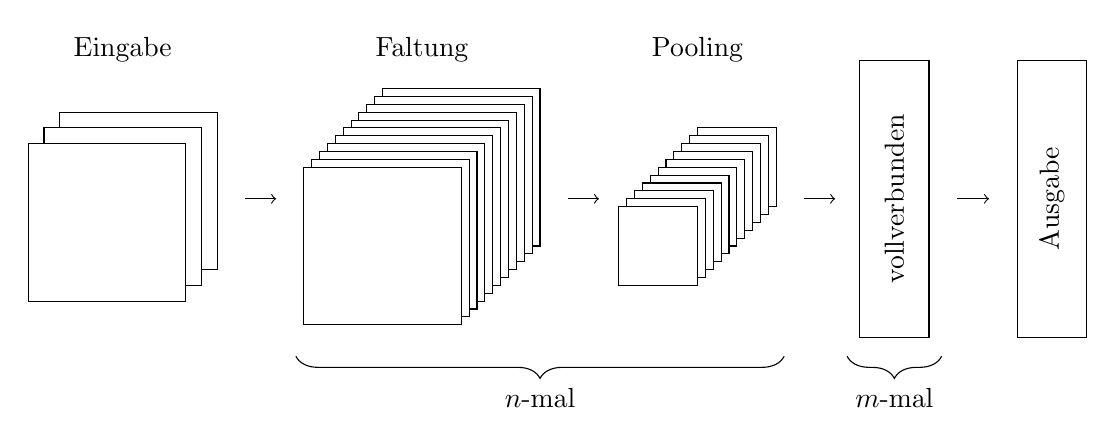
\begin{tikzpicture}
  \tikzstyle{node}=[rectangle, draw, minimum width=100pt, minimum height=25pt, inner sep=0pt, fill=white, rotate=90]
  \tikzstyle{rect}=[rectangle, draw, fill=white]
  \tikzstyle{path}=[->, shorten >= 10pt, shorten <= 10pt]

  % Eingabe.
  \draw[rect] (-0.1, 0.4) rectangle (1.9, 2.4);
  \draw[rect] (-0.3, 0.2) rectangle (1.7, 2.2);
  \draw[rect] (-0.5, 0)   rectangle (1.5, 2);

  % Faltung.
  \draw[rect] (4,   0.7)  rectangle (6,   2.7);
  \draw[rect] (3.9, 0.6)  rectangle (5.9, 2.6);
  \draw[rect] (3.8, 0.5)  rectangle (5.8, 2.5);
  \draw[rect] (3.7, 0.4)  rectangle (5.7, 2.4);
  \draw[rect] (3.6, 0.3)  rectangle (5.6, 2.3);
  \draw[rect] (3.5, 0.2)  rectangle (5.5, 2.2);
  \draw[rect] (3.4, 0.1)  rectangle (5.4, 2.1);
  \draw[rect] (3.3, 0)    rectangle (5.3, 2);
  \draw[rect] (3.2, -0.1) rectangle (5.2, 1.9);
  \draw[rect] (3.1, -0.2) rectangle (5.1, 1.8);
  \draw[rect] (3,   -0.3) rectangle (5, 1.7);

  % Pooling.
  \draw[rect] (8,   1.2) rectangle (9,   2.2);
  \draw[rect] (7.9, 1.1) rectangle (8.9, 2.1);
  \draw[rect] (7.8, 1)   rectangle (8.8, 2);
  \draw[rect] (7.7, 0.9) rectangle (8.7, 1.9);
  \draw[rect] (7.6, 0.8) rectangle (8.6, 1.8);
  \draw[rect] (7.5, 0.7) rectangle (8.5, 1.7);
  \draw[rect] (7.4, 0.6) rectangle (8.4, 1.6);
  \draw[rect] (7.3, 0.5) rectangle (8.3, 1.5);
  \draw[rect] (7.2, 0.4) rectangle (8.2, 1.4);
  \draw[rect] (7.1, 0.3) rectangle (8.1, 1.3);
  \draw[rect] (7,   0.2) rectangle (8,   1.2);

  \node at (0.7, 3.2) {Eingabe};
  \node at (4.5, 3.2) {Faltung};
  \node at (8,   3.2) {Pooling};

  \node[node] (1)  at (10.5, 1.3) {vollverbunden};
  \node[node] (2)  at (12.5, 1.3) {Ausgabe};

  \path[path] (1.9, 1.3) edge (3,    1.3);
  \path[path] (6, 1.3)   edge (7.1,  1.3);
  \path[path] (9, 1.3)   edge (10.1, 1.3);

  \path[path] (1) edge (2);

  \draw [decoration={brace,mirror,amplitude=8pt},decorate,-] (2.9,-0.7) -- node[below=8pt] {$n$-mal} (9.1,-0.7);
  \draw [decoration={brace,mirror,amplitude=8pt},decorate,-] (9.9,-0.7) -- node[below=8pt] {$m$-mal} (11.1,-0.7);
\end{tikzpicture}
  \caption[Netzarchitektur eines \glspl{CNN}]{Typische Netzarchitektur eines \glspl{CNN} bestehend aus beliebig vielen Faltungs- gefolgt von Poolingschichten.
  Die Abflachung der Merkmalskarten zu einem Vektor erlaubt die Verwendung beliebig vieler vollverbundener Schichten hin zur Ausgabe.}
\label{fig:cnn_aufbau}
\end{figure}


